\documentclass[10pt,a4paper]{article}
\usepackage[latin1]{inputenc}
\usepackage{amsmath}
\usepackage{amsfonts}
\usepackage{amssymb}
\usepackage{float}
\usepackage{listings}
\usepackage{graphicx}

\begin{document}

\lstset{language=Python,breaklines=true}

\author{Jeroen Hofman\\
		10194754\\
		}
\title{Computer exercises week 37,2011\\
		}
\date{}
\maketitle

\subsection*{Exercise 2.2}

Code:
\begin{lstlisting}
#PLU factorization of A
(P,L,U) = lu(A)

#Solve PLy = b
L = np.dot(P,L)
y[0] = b[1]/L[1,0]
y[1] = (b[2] - L[2,0]*y[0])/L[2,1]
y[2] = (b[0] - L[0,0]*y[0] - L[0,1]*y[1])/L[0,2]

#Solve Ux = y
x[2] = y[2]/U[2,2]
x[1] = (y[1] - U[1,2]*x[2])/U[1,1]
x[0] = (y[0] - U[0,1]*x[1] - U[0,2]*x[2])/U[0,0]

#2.2c Take u = (1,0,0)^T and v = (0,2,0), then solve Az = PLUz = u
#Solve PLq = u
q[0] = u[1]/L[1,0]
q[1] = (u[2] - L[2,0]*q[0])/L[2,1]
q[2] = (u[0] - L[0,0]*q[0] - L[0,1]*q[1])/L[0,2]

#Solve Uz = q
z[2] = q[2]/U[2,2]
z[1] = (q[1] - U[1,2]*z[2])/U[1,1]
z[0] = (q[0] - U[0,1]*z[1] - U[0,2]*z[2])/U[0,0]

x = x + np.dot(v,x)/(1-np.dot(v,z)) * z
\end{lstlisting}

\noindent In this exercise we solve the problem with Gaussian elimination, using an algorithm from the numpy package in Python, which gives an PLU decomposition of A from which we can solve Ax = b. Using the code above we first solve PLy = b and then Ux = y, the result is x = \{13,6,-2\}$^T$. After this we just substitute another vector c instead of b without changing the PLU decomposition, giving x = \{-1,1,-1\}$^T$. For 2c we use the Sherman-Morrison updating technique by taking u = \{1,0,0\}$^T$ and v = \{0,2,0\}, then the new matrix is A-u$^{T}$v. The solution is then given by x = x+$\frac{v^T x}{1-v^T z} z$, where z is the solution of Az = u. Using this method we obtain x = \{2,1/2,3/2\}$^T$.

\subsection*{Exercise 2.6}

code:
\begin{lstlisting}
while n<14:
    
#generate Hilbert matrix of order n
    for i in range (0,n):
        for j in range (0,n):
            A[i,j] = 1/(-1+(float(i)+1)+(float(j)+1))

    xsol = np.array(np.ones([n]))
    b = np.dot(A,xsol)

#Perform cholesky algorithm
    L  = cholesky(A)

#solve Ly = b
    while k < n:
        y[k] = b[k]
        for l in range(0,k):
            y[k] -= L[k,l]*y[l]
        y[k] = y[k]/L[k,k]
        k += 1

#solve L^Tx = y
    U = np.transpose(L)
    k = n -1
    while k > -1:
        x[k] = y[k]
        for l in range(k+1,n):
            x[k] -= U[k,l]*x[l]
        x[k] = x[k]/U[k,k]
        k -= 1
    
#compute errors
    delta = x - xsol
    r = b - np.dot(A,x)
    residual,error = 0,0
    for j in range (0,n):
        residual+=abs(r[j])
        error+=abs(delta[j])
\end{lstlisting}

\noindent In this exercise the Hilbert matrix H was generated for n=3 up to n=13. We compute b = Hx, where x is a column vector of length n with all components equal to 1. Then we compute $\hat{x}$ by solving the linear system H$\hat{x}$ = b. We solve this systems using a Cholesky factorization, which is a numpy package and gives us an upper triangle matrix L such that LL$^T$ = A. We then solve $\hat{x}$ by first computing Ly = b and then L$^T \hat{x}$ = y. We compute the infinity norm of $\Delta x$ = $\hat{x}$-x and the infinity norm of b - H$\hat{x}$, the results for $\Delta x$ are shown in the figure below. For small matrices the errors are relatively small, but the error in $\hat{x}$ increases every step by a factor of 100. When n=12 the error in $\hat{x}$ is bigger than 1 and hence the error is very big. I couldn't compute further than n=13 (the error is about 10) because then my algorithm wouldn't do the Cholesky factorization anymore, since the matrix it was generating was not symmetric anymore because of rounding. It is remarkable that although the error in $\hat{x}$ grows very fast, the error in b - H$\hat{x}$ grows much slower and is still very small ($\approx$ 10$^{-10}$) at n=13.

\begin{figure}[H]
\centering
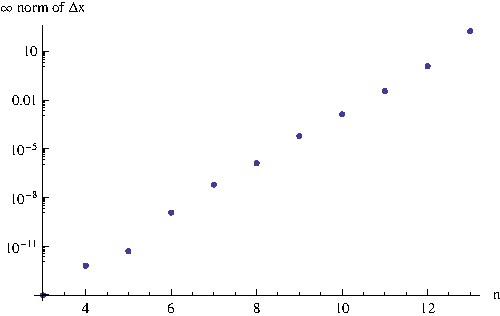
\includegraphics[scale=1.0]{2_6.pdf}
\end{figure}

\subsection*{Exercise 3.1}

Code:
\begin{lstlisting}
t = np.array([0.0,1.0,2.0,3.0,4.0,5.0])

n=1;
while n < 7:
    b = np.array([[1.0],[2.7],[5.8],[6.6],[7.5],[9.9]])
    for i in range(0,6):
        for j in range(0,n):
            A[i,j]=t[i]**j
    b = np.dot(np.transpose(A),b)
    A = np.dot(np.transpose(A),A)
    L = cholesky(A)

#solve Ly = b
    while k < n:
        y[k] = b[k]
        for l in range(0,k):
            y[k] -= L[k,l]*y[l]
        y[k] = y[k]/L[k,k]
        k += 1

#solve L^Tx = y
    U = np.transpose(L)
    k = n -1
    while k > -1:
        x[k] = y[k]
        for l in range(k+1,n):
            x[k] -= U[k,l]*x[l]
        x[k] = x[k]/U[k,k]
        k -= 1
\end{lstlisting}

\noindent In this exercise we used the least squared method to fit a curve through a dataset. We first set up the linear equations Ax = b, where x is the array with the desired coefficients for the fit, a$_{i,j}$ = $t_{i}^{j}$, where $t_{i}$ is the i-th data point of t and $b_{i}$ the ith data point of y. Then we calculate A$^T$Ax = A$^T$b. We define A$^T$b = $\hat{b}$ and $\hat{A}$ = A$^T$A, since A$^T$A is positive definite, we use a Cholesky factorization algorithm to solve for x. The figure below shows the results of the fit of different orders (up to 5), the red line gives the best approximation, which is a polynomial of order 5. It clearly intersects with most of the data points and seems to follow the path one would choose by interpolating the data points. In general, the smaller the order of the polynomial that is fitted, the worse the actual fit is, as can be seen clearly in the figure below.

\begin{figure}[H]
\centering
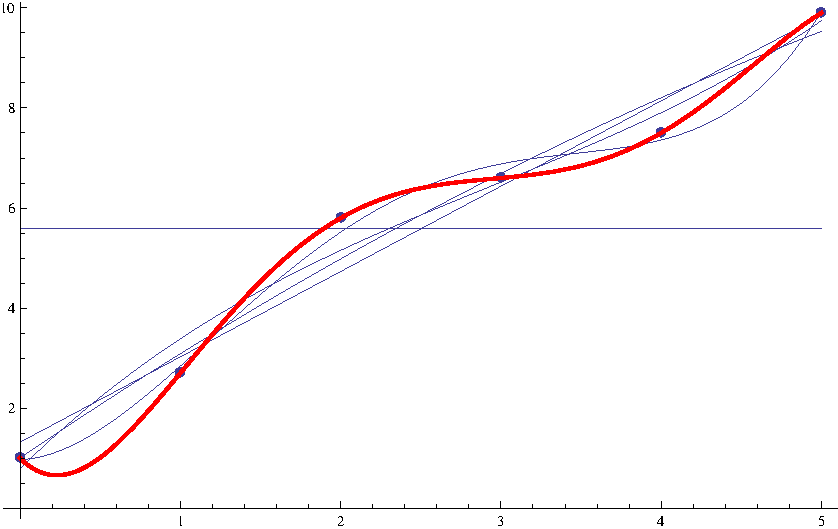
\includegraphics[scale=0.5]{3_1.pdf}
\end{figure}


\subsection*{Exercise 3.3a}

Code:
\begin{lstlisting}
time=0
n=100
while n < 1000:
    for i in range(0,50):
        t = timeit.Timer("(P,L,U) = lu(A)","import numpy as np; from scipy.linalg import lu; \\A = np.matrix(np.random.randn("+str(n)+","+str(n)+"))")
        time += t.timeit(1)
        if i == 49:
            time = time/50
    n+=100
\end{lstlisting}

\noindent In the last exercise we measured the time to perform an LU decomposition of random matrices of various sizes. We started with a 100x100 matrix up to a 900x900 matrix in steps of n=100. We performed the time measurement at every n 50 times with randomly generated matrices, see the code above. I used the LeastSquares routine in Mathematica to fit the results to a cubic polynomial. The input matrix A = \{\{1,100,100$^2$,100$^3$\},\{1,200,200$^{2}$... etc\}\} and the vector t = \{t$_{n=100}$,t$_{n=200}$...etc\} are used to solve Ax = t, where the x vector gives the coefficients of the powers of n. Using this method we found that time(LU(n)) $\approx$ 0.000712562 - 3.21703 10$^{-6}$ x + 7.78175 10$^{-8}$ x$^2$ + 1.40078 10$^{-9}$ x$^3$, see also the figure below. Using this numbers we obtain a predicted execution time for order 10000 of approximately 1409 seconds.

\begin{figure}[H]
\centering
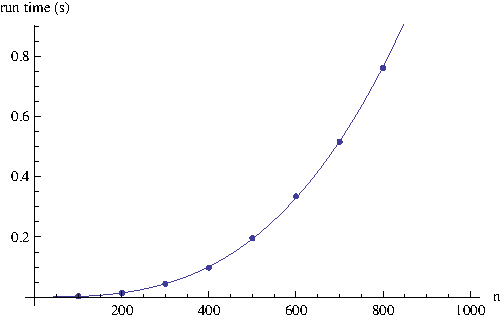
\includegraphics[scale=1.0]{3_3.pdf}
\end{figure}

\end{document}